\chapter{COLREGS Compliant Guidance System}
\label{chap:4_COLREGS_Compliant_Guidance_System}

    Is this chapter we present and describe the architecture of the \ac{USV} system we developed.

\section{Assumptions and Limitations}

    \begin{enumerate}
        
        %%%%%%%%%%%%%%%%%%%%%%%%
        % Grammarly: 100/100
        %%%%%%%%%%%%%%%%%%%%%%%%
        \item Encountering between power-driven vessels: we developed our system to run on power-driven vessels and considered the encountering between vessels of the same type. Concerning COLREGS, the encounter between different types of vessels imposes different ways to avoid collisions. Our system, in its current state, may be able to avoid collision with other vessels, but the avoidance strategy will always consider the other vessel as a power-driven vessel.

        %%%%%%%%%%%%%%%%%%%%%%%%
        % Grammarly: 95/100
        %%%%%%%%%%%%%%%%%%%%%%%%
        \item Encountering with one vessel: currently, we developed our system to perform COLREGS-compliant collision avoidance with only one vessel at a time. In a multiple vessels encounter scenario, our system may be able to perform evasive actions but we do not have any assurance regarding COLREGS-compliance for this scenario.

    \end{enumerate}

\section{System Architecture}

    %%%%%%%%%%%%%%%%%%%%%%%%
    % Grammarly: 100/100
    %%%%%%%%%%%%%%%%%%%%%%%%
    Our system consists of 3 main modules: guidance, navigation, and control. In Figure \ref{fig:gnc_arch}, we present an overview of the system.
    %Além dos módulos que compõem o nosso sistema são apresentados módulos externos ao \ac{USV} que são responsáveis pelo comportamento simulado do USV\_SIM e pelo 

    \begin{figure}
        \centering
        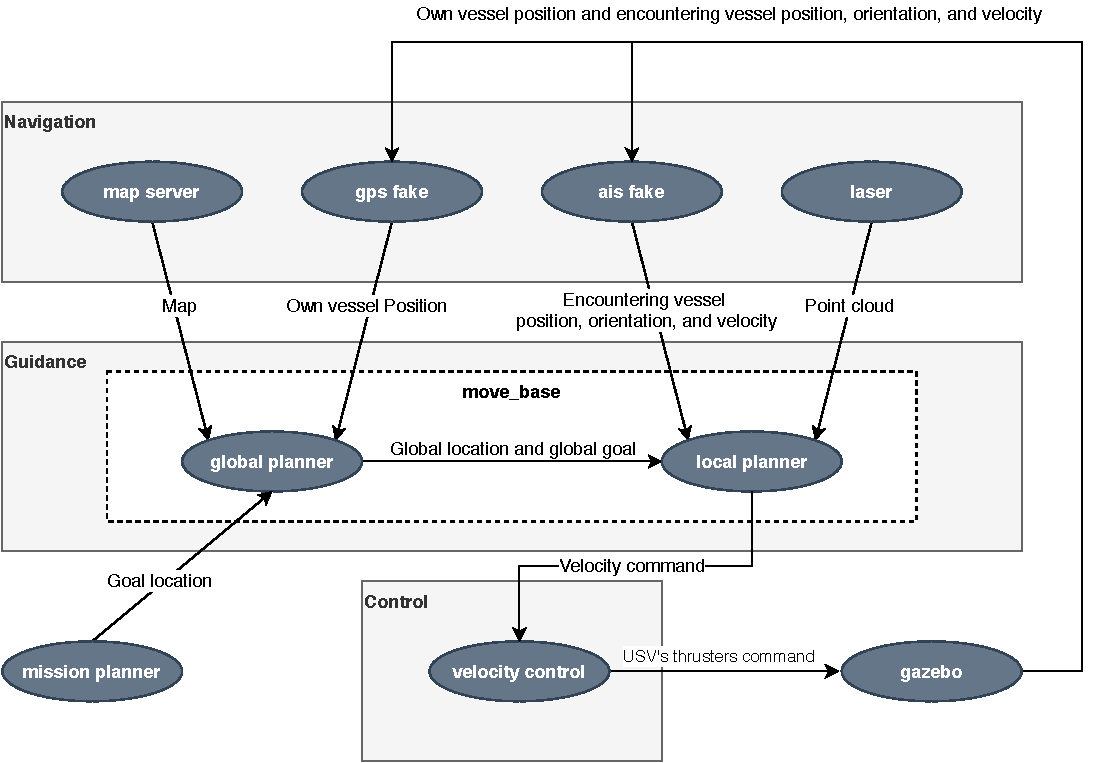
\includegraphics[scale=0.75]{figs/Chap4/gnc_arch.pdf}
        %%%%%%%%%%%%%%%%%%%%%%%%
        % Grammarly: 100/100
        %%%%%%%%%%%%%%%%%%%%%%%%
        \caption{Guidance, Navigation, and Control System Architecture: Beyond the GNC components of our system, we show in this Figure the mission\_planner and gazebo modules. The mission\_planner module is responsible for generating location goals to be followed by our \ac{USV}. The mission\_planner is currently an independent ROS-package; we developed it as an external module; this way, it can be replaced by any other module compliant to ROS publishing. The gazebo module is a general module for interacting with the simulator; through it, we can change and gather the \ac{USV} and the environment state.}
        \label{fig:gnc_arch}
    \end{figure}
    
    \subsection{Guidance}
    
        As shown in Figure \ref{fig:gnc_arch} the guidance module is mainly composed of global and local planner. Both planners are implemented inside the ROS move\_base environment. Fr global planning we use the move\_base standard A* search and for local planning we developed our own ROS move\_base plugin. This way we created our COLREGS-compliant local path planner and kept ROS compatibility.

        \subsubsection{Local Planner}
        
            %%%%%%%%%%%%%%%%%%%%%%%%
            % Grammarly: 99/100
            %%%%%%%%%%%%%%%%%%%%%%%%
            The local planner module is responsible for the reactive behavior of the system; that is, when encountering unknown static or dynamic obstacles, this module must be able to generate a behavior to avoid collision and, if possible, stay aligned with the global route generated by the global planner module.
        
            %%%%%%%%%%%%%%%%%%%%%%%%
            % Grammarly: 99/100
            %%%%%%%%%%%%%%%%%%%%%%%%
            In our system, the local planner module is responsible for COLREGS-compliant path planning. For COLREGS compliance, we adapted the usage of \ac{ATC} as presented by Agrawal \etal~\cite{Agrawal2015COLREGS}. With \ac{ATC}, we restrict the search space, building virtual obstacles in no COLREGS-compliant locations, see Figure \ref{fig:atc}.
            
            \begin{figure}[H]
            \centering
            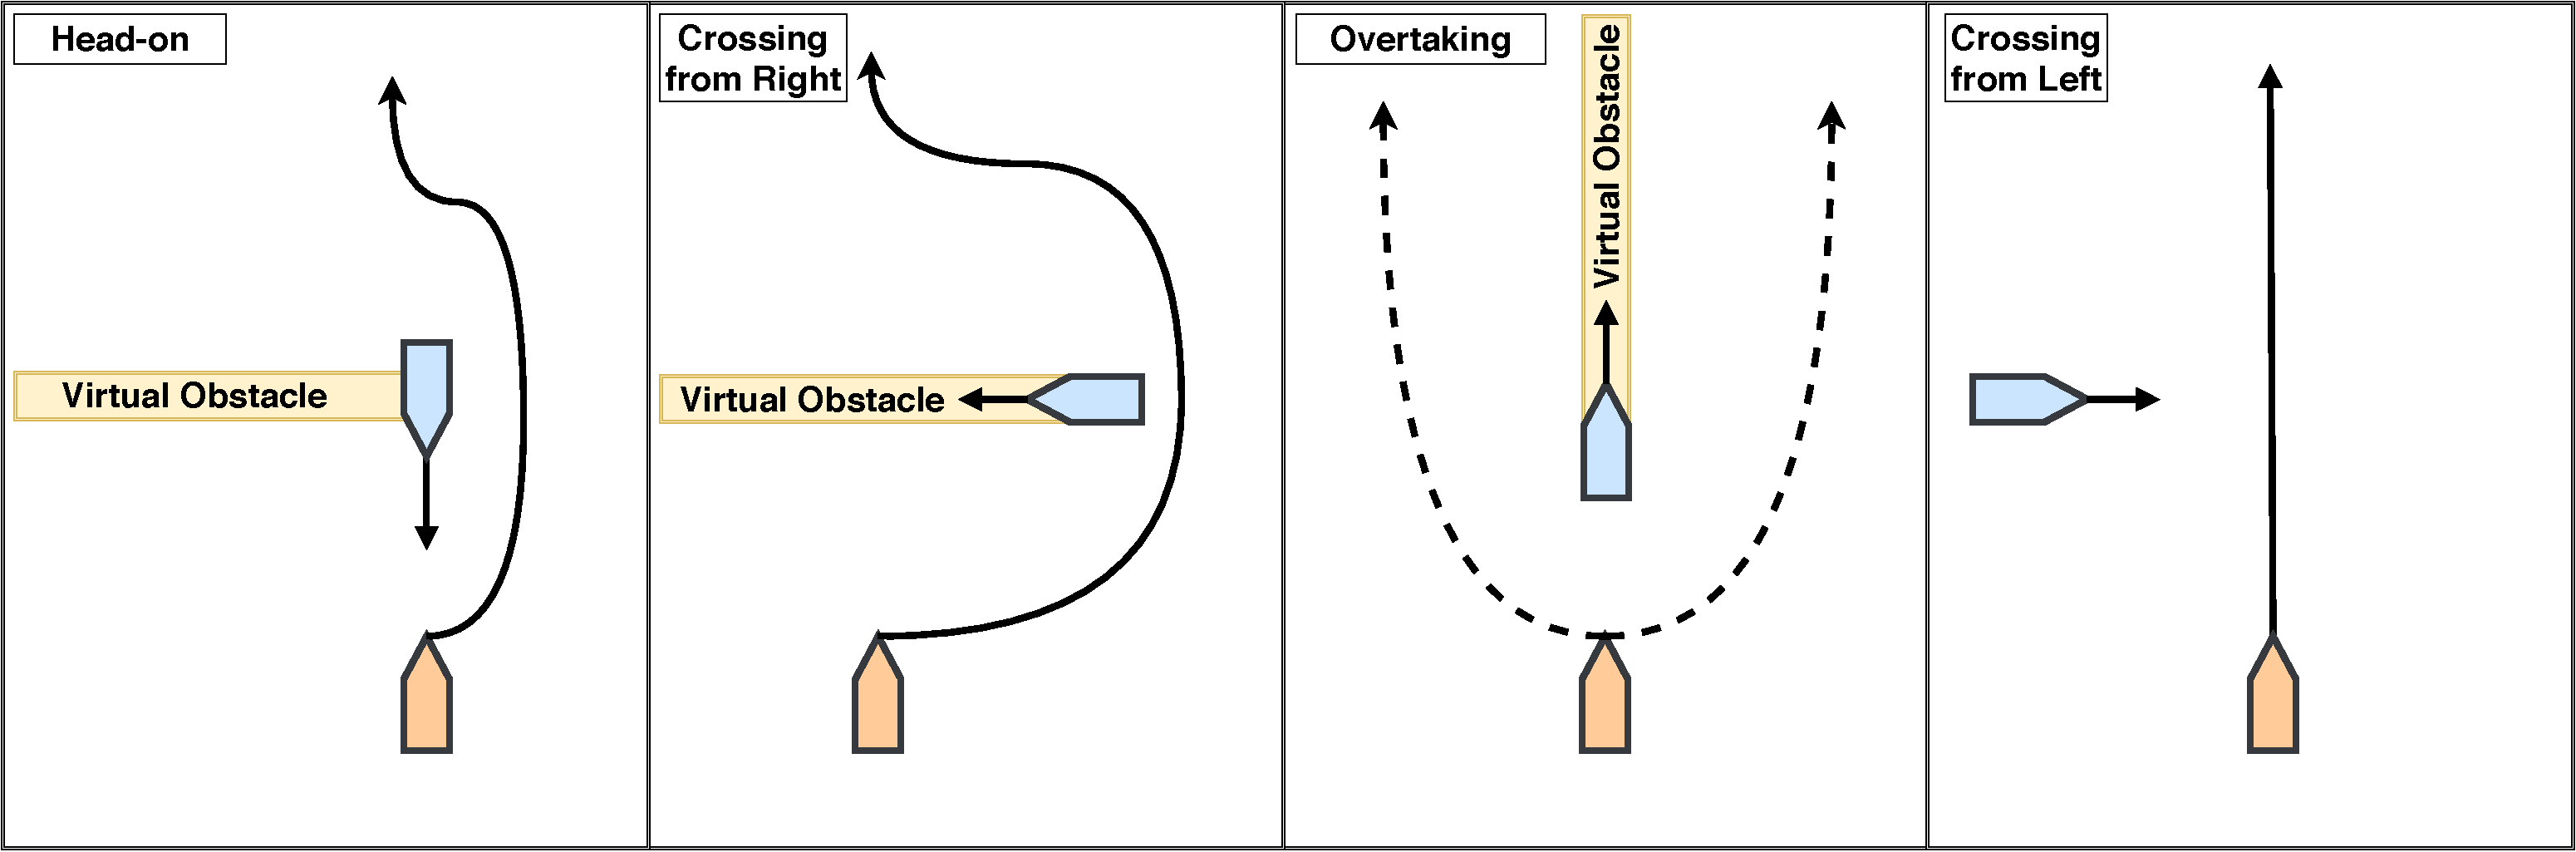
\includegraphics[scale=0.32]{figs/Chap4/atc.pdf}
            %%%%%%%%%%%%%%%%%%%%%%%%
            % Grammarly: 100/100
            %%%%%%%%%%%%%%%%%%%%%%%%
            \caption{\ac{ATC} for COLREGS Encounters: }
            \label{fig:gnc_arch}
        \end{figure}
        
        \begin{figure}[H]
            \centering
            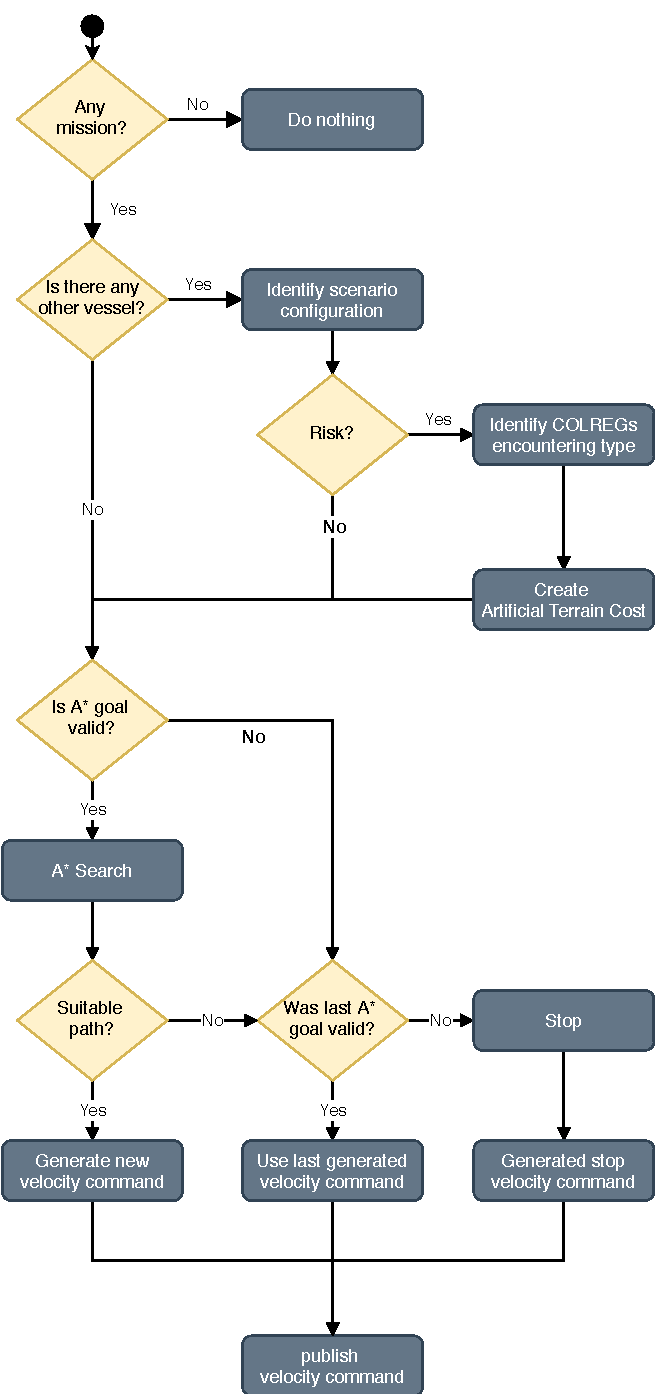
\includegraphics[scale=0.75]{figs/Chap4/AStartwithATC_flowChart.pdf}
            %%%%%%%%%%%%%%%%%%%%%%%%
            % Grammarly: 100/100
            %%%%%%%%%%%%%%%%%%%%%%%%
            \caption{Here we present a simplification of the sequential execution of our COLREGS-compliant path planning method. Some details are omitted to facilitate the general understanding of how our method works.}
            \label{fig:gnc_arch}
        \end{figure}

    \subsection{Navigation}
    The navigation system consists of the following sub-modules:
    
    \begin{itemize}
    
        %%%%%%%%%%%%%%%%%%%%%%%%
        % Grammarly: 99/100
        %%%%%%%%%%%%%%%%%%%%%%%%
        \item \textbf{map\_server}: the map\_server module is responsible for making the global map available for the guidance system. The map is generated before the start of the \ac{USV} mission. Both the map and an adapted version of the map\_server module were made available by the USV\_SIM maintainers.
    
        %%%%%%%%%%%%%%%%%%%%%%%%
        % Grammarly: 99/100
        %%%%%%%%%%%%%%%%%%%%%%%%
        \item \textbf{gps\_fake}: the gps\_fake module is a simplification of a real GPS; its information is extracted directly from the simulator; that is, it does not perform a simulated query to satellites. The gps\_fake module performs a simple query to the gazebo module in order to acquire a 3-tuple for determination of the position of the \ac{USV} in the global reference plane. This module can be replaced by another localization method, such as AMCL or a real GPS device. We developed and integrated this module into the system as a contribution to this work.
    
        %%%%%%%%%%%%%%%%%%%%%%%%
        % Grammarly: 99/100
        %%%%%%%%%%%%%%%%%%%%%%%%
        \item \textbf{ais\_fake}: the ais\_fake module is a simplification of the real AIS system \footnote{A real AIS module must respect NMEA legislation, refer to NMEA for specification: URL} which is used on vessels sailing on the high seas. The ais\_fake module provides the position and velocity of another vessel. The ais\_fake generate its information from a direct query to the simulator data. We developed and integrated this module into the system as a contribution to this work.
    
        %%%%%%%%%%%%%%%%%%%%%%%%
        % Grammarly: 100/100
        %%%%%%%%%%%%%%%%%%%%%%%%
        \item \textbf{laser}: this module provides the location of bodies of mass that reflect the laser light beam through an ordered 3-tuple. This module is available as a standard module in USV\_SIM. We configured this module to be compatible with the following requirements: laser beam range up to 25m and 360º detection capability; both specifications are compatible with real lasers, for example, the Slamtec RPLIDAR A3 laser \cite{RPLidarA3}.
    
    \end{itemize}
    
    % \subsection{Guidance}
    % O sistema de guidance é composto pelos seguintes submódulos:
    % \begin{itemize}
    %     \item \textbf{global\_planner}: O módulo global\_planner é responsável por .
    %     \item \textbf{local\_planner}: .
    % \end{itemize}
    
    \subsection{Control}
    
        %%%%%%%%%%%%%%%%%%%%%%%%
        % Grammarly: 100/100
        %%%%%%%%%%%%%%%%%%%%%%%%
        The control system consists of the control\_vel module. The control\_vel module interacts directly with the simulator and sends actuation commands to modify the state of \ac{USV}. The control\_vel module sends actuation commands from the speed commands received from the local planning module. This module is available as a standard module in USV\_SIM, and we used it without any modifications.


    
% VO because the algorithms collect all the velocities that result in collisions and present a set of collision-free velocities for human/machine, which facilitates human/machine to search for the best option.

% The advantages of the VO algorithms have been noticed by researchers in maritime engineering. The idea of VO algorithms had ap- peared in the 1980s, named as Collision Threat Parameter Area (CTPA) (Degre and Lefevre, 1981; Lenart, 1983). Subsequently, Pedersen et al. (2003) showed that this method can provide a better support for the Officer On Watch (OOW) in collision prevention comparing with tra- ditional Automatic Radar Plotting Aid (ARPA). Later on, a series of studies proposed to use VO/CTPA algorithms for collision avoidance in various scenarios, e.g. restricted waters (Szlapczynski and Szlapczynska, 2017), multiple-ship (Szlapczynski, 2008), incorporating with regulations (Zhao et al., 2016), and unmanned ship (Kuwata et al., 2014). In (Huang et al., 2018), the algorithms which presume the target-ship keeps constant velocity, are concluded as a special case of the VO algorithm, called linear VO (LVO) algorithm. Details about the existing applications of VO algorithms in the maritime domain are addressed in Section 2.3.